% Diagrama de Sistema de Control Jerárquico con TikZ
% Puedes compilar este archivo independientemente o incluirlo en el documento principal

\documentclass[tikz,border=10pt]{standalone}
\usepackage{tikz}
\usetikzlibrary{shapes.geometric, arrows.meta, positioning, calc, fit, backgrounds}

\begin{document}

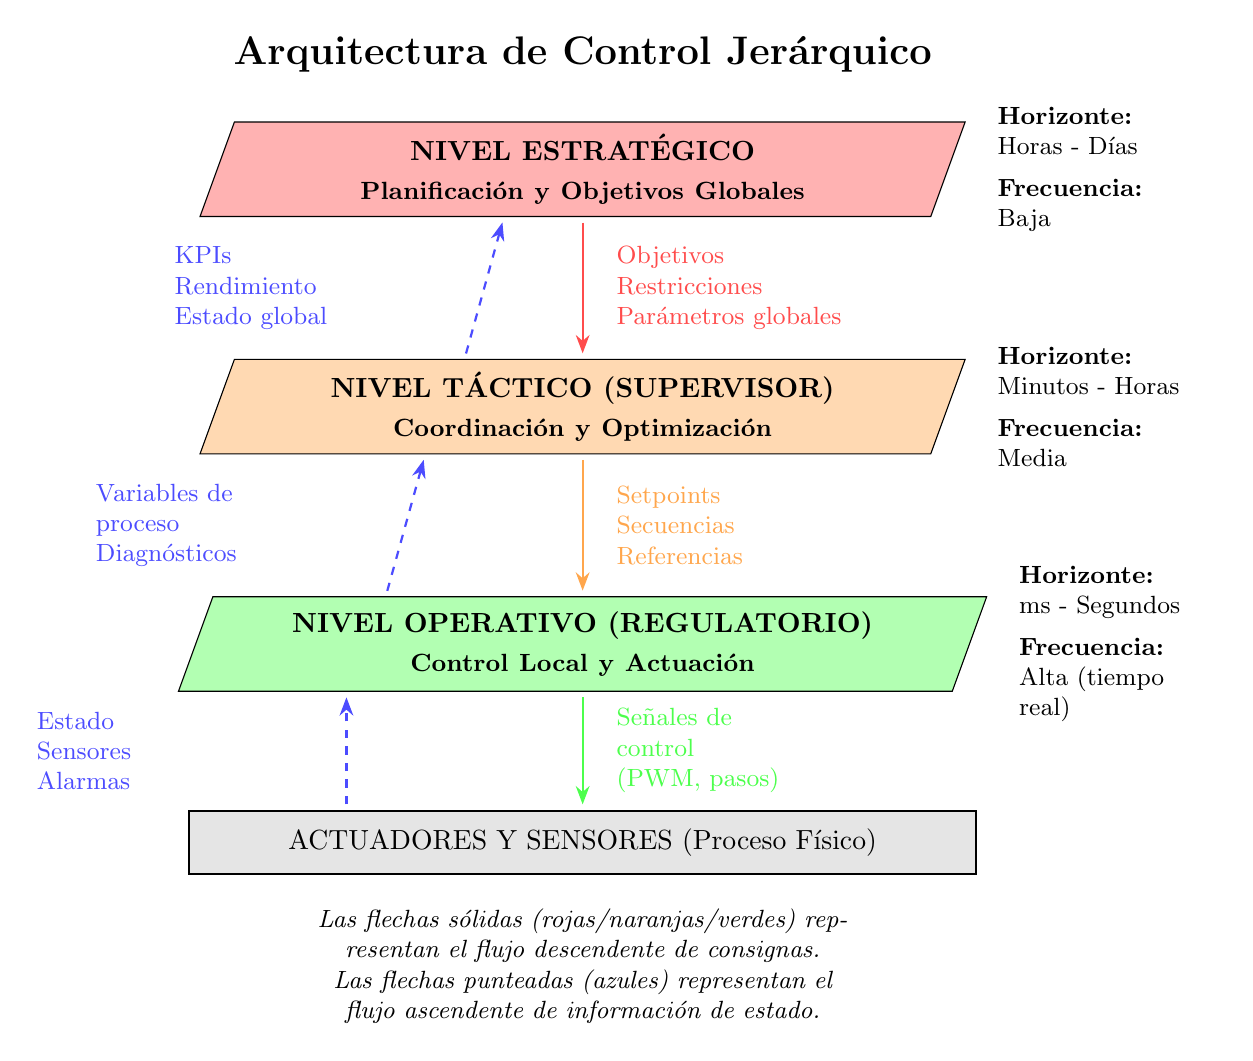
\begin{tikzpicture}[
    node distance=1.5cm,
    nivel/.style={
        trapezium,
        trapezium left angle=70,
        trapezium right angle=110,
        minimum width=3cm,
        minimum height=1.2cm,
        text centered,
        draw=black,
        fill=blue!20,
        font=\bfseries,
        text width=8cm,
        align=center
    },
    flecha/.style={
        -Stealth,
        thick,
        shorten >=2pt,
        shorten <=2pt
    },
    info/.style={
        font=\small,
        text width=3.5cm,
        align=left
    }
]

% Niveles de la jerarquía
\node (estrategico) [nivel, fill=red!30, minimum width=4cm]
    {NIVEL ESTRATÉGICO\\[2pt]\small Planificación y Objetivos Globales};

\node (tactico) [nivel, fill=orange!30, below=1.8cm of estrategico, minimum width=7cm]
    {NIVEL TÁCTICO (SUPERVISOR)\\[2pt]\small Coordinación y Optimización};

\node (operativo) [nivel, fill=green!30, below=1.8cm of tactico, minimum width=10cm]
    {NIVEL OPERATIVO (REGULATORIO)\\[2pt]\small Control Local y Actuación};

% Bloques inferiores (actuadores/sensores)
\node (actuadores) [below=1.5cm of operativo,
                    draw=black, thick, fill=gray!20,
                    minimum width=10cm, minimum height=0.8cm,
                    text centered]
    {ACTUADORES Y SENSORES (Proceso Físico)};

% Flechas de consignas (descendentes)
\draw[flecha, red!70] (estrategico.south) -- (tactico.north)
    node[midway, right=0.3cm, info] {Objetivos\\Restricciones\\Parámetros globales};

\draw[flecha, orange!70] (tactico.south) -- (operativo.north)
    node[midway, right=0.3cm, info] {Setpoints\\Secuencias\\Referencias};

\draw[flecha, green!70] (operativo.south) -- (actuadores.north)
    node[midway, right=0.3cm, info] {Señales de\\control\\(PWM, pasos)};

% Flechas de realimentación (ascendentes)
\draw[flecha, blue!70, dashed] ([xshift=-3cm]actuadores.north) -- ([xshift=-3cm]operativo.south)
    node[midway, left=0.3cm, info] {Estado\\Sensores\\Alarmas};

\draw[flecha, blue!70, dashed] ([xshift=-2.5cm]operativo.north) -- ([xshift=-2cm]tactico.south)
    node[midway, left=0.3cm, info] {Variables de\\proceso\\Diagnósticos};

\draw[flecha, blue!70, dashed] ([xshift=-1.5cm]tactico.north) -- ([xshift=-1cm]estrategico.south)
    node[midway, left=0.3cm, info] {KPIs\\Rendimiento\\Estado global};

% Escalas temporales
\node[right=0.5cm of estrategico, info, text width=2.5cm]
    {\textbf{Horizonte:}\\Horas - Días\\[4pt]\textbf{Frecuencia:}\\Baja};

\node[right=0.5cm of tactico, info, text width=2.5cm]
    {\textbf{Horizonte:}\\Minutos - Horas\\[4pt]\textbf{Frecuencia:}\\Media};

\node[right=0.5cm of operativo, info, text width=2.5cm]
    {\textbf{Horizonte:}\\ms - Segundos\\[4pt]\textbf{Frecuencia:}\\Alta (tiempo real)};

% Título
\node[above=0.5cm of estrategico, font=\Large\bfseries]
    {Arquitectura de Control Jerárquico};

% Leyenda
\node[below=0.3cm of actuadores, font=\small\itshape, text width=10cm, align=center]
    {Las flechas sólidas (rojas/naranjas/verdes) representan el flujo descendente de consignas.\\
     Las flechas punteadas (azules) representan el flujo ascendente de información de estado.};

\end{tikzpicture}

\end{document}
